\documentclass{article}
\usepackage[paperwidth=14cm,paperheight=8cm,margin=0.2cm]{geometry}
\usepackage{amsmath,amssymb}
\usepackage{xcolor}
\usepackage{tikz}
\usetikzlibrary{arrows.meta,positioning,calc,fit,shapes.geometric,backgrounds}

\begin{document}
\pagestyle{empty}
\centering

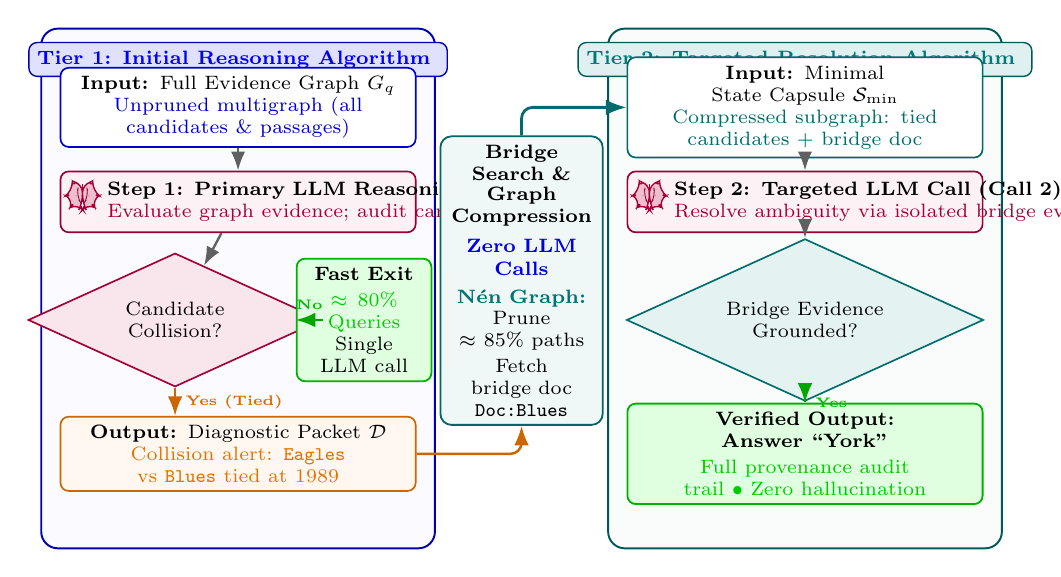
\begin{tikzpicture}[
  >=Latex,
  font=\sffamily\scriptsize,
  % Panels
  panel/.style={draw=#1!70!black, fill=#1!2!white, rounded corners=6pt, line width=0.7pt},
  panel_hdr/.style={fill=#1!12, draw=#1!70!black, line width=0.5pt, rounded corners=3pt, font=\bfseries\scriptsize, text=#1!95!black, inner sep=3pt, align=center},
  % Flowchart Nodes
  fc_input/.style={draw=#1!80!black, fill=white, rounded corners=3pt, line width=0.6pt, inner sep=3pt, align=center, font=\scriptsize},
  fc_proc/.style={draw=purple!80!black, fill=purple!5, rounded corners=3pt, line width=0.6pt, inner sep=3pt, align=center, font=\scriptsize},
  fc_dec/.style={diamond, aspect=2.2, draw=#1!85!black, fill=#1!10, line width=0.6pt, inner sep=1.5pt, align=center, font=\scriptsize},
  fc_exit/.style={draw=green!70!black, fill=green!12, rounded corners=3pt, line width=0.65pt, inner sep=3pt, align=center, font=\scriptsize},
  fc_out/.style={draw=orange!80!black, fill=orange!6, rounded corners=3pt, line width=0.6pt, inner sep=3pt, align=center, font=\scriptsize},
  % Bridge Box
  bridge_style/.style={draw=teal!80!black, fill=teal!6, rounded corners=4pt, line width=0.65pt, inner sep=3pt, align=center, font=\scriptsize},
  % Arrows
  arr/.style={->, line width=0.85pt, draw=gray!75!black},
  arr_green/.style={->, line width=0.9pt, draw=green!65!black},
  arr_orange/.style={->, line width=0.9pt, draw=orange!80!black},
  arr_bridge/.style={->, line width=1.0pt, draw=teal!85!black}
]

% Brain icon pic
\tikzset{
  brain/.pic={
    \begin{scope}[scale=0.18]
      \draw[fill=purple!25, draw=purple!85!black, line width=0.5pt]
        (0, 0.72) 
        .. controls (-0.35, 0.82) and (-0.72, 0.62) .. (-0.72, 0.28)
        .. controls (-0.92, 0.12) and (-0.92, -0.22) .. (-0.68, -0.34)
        .. controls (-0.76, -0.58) and (-0.52, -0.78) .. (-0.28, -0.68)
        .. controls (-0.18, -0.82) and (-0.05, -0.68) .. (0, -0.58)
        -- cycle;
      \draw[fill=purple!25, draw=purple!85!black, line width=0.5pt]
        (0, 0.72) 
        .. controls (0.35, 0.82) and (0.72, 0.62) .. (0.72, 0.28)
        .. controls (0.92, 0.12) and (0.92, -0.22) .. (0.68, -0.34)
        .. controls (0.76, -0.58) and (0.52, -0.78) .. (0.28, -0.68)
        .. controls (0.18, -0.82) and (0.05, -0.68) .. (0, -0.58)
        -- cycle;
      \draw[purple!85!black, line width=0.5pt] (0, 0.70) -- (0, -0.56);
      \fill[purple!85!black] (-0.35, 0.3) circle (0.8pt);
      \fill[purple!85!black] (-0.45, -0.1) circle (0.8pt);
      \fill[purple!85!black] (-0.25, -0.4) circle (0.8pt);
      \draw[purple!70!black, line width=0.3pt] (-0.35, 0.3) -- (-0.45, -0.1) -- (-0.25, -0.4);
      \fill[purple!85!black] (0.35, 0.3) circle (0.8pt);
      \fill[purple!85!black] (0.45, -0.1) circle (0.8pt);
      \fill[purple!85!black] (0.25, -0.4) circle (0.8pt);
      \draw[purple!70!black, line width=0.3pt] (0.35, 0.3) -- (0.45, -0.1) -- (0.25, -0.4);
    \end{scope}
  }
}

% GEOMETRY:
% Left Panel (Tier 1): X center = 2.6cm, Width = 5.0cm
% Right Panel (Tier 2): X center = 9.8cm, Width = 5.0cm
% Gap between panels: X from 5.1 to 7.3 (width 2.2cm, center 6.2cm)

% -------------------------------------------------------------
% TIER 1 PANEL
% -------------------------------------------------------------
\node[panel=blue, minimum width=5.0cm, minimum height=6.6cm] (p1) at (2.6, 0) {};
\node[panel_hdr=blue, minimum width=4.7cm, anchor=north] (p1_title) at ([yshift=-1.8mm]p1.north) {
  Tier 1: Initial Reasoning Algorithm
};

% T1 Step 1: Input
\node[fc_input=blue, text width=4.3cm] (t1_in) at (2.6, 2.3) {
  \textbf{Input:} Full Evidence Graph $G_q$\\
  \textcolor{blue!80!black}{Unpruned multigraph (all candidates \& passages)}
};

% T1 Step 2: LLM Process
\node[fc_proc, text width=4.3cm] (t1_llm) at (2.6, 1.1) {
  \begin{tabular}{@{}c@{\hspace{4pt}}l@{}}
    \tikz{\pic {brain};} &
    \begin{tabular}{@{}l@{}}
      \textbf{Step 1: Primary LLM Reasoning (Call 1)}\\
      \textcolor{purple!85!black}{Evaluate graph evidence; audit candidate clarity}
    \end{tabular}
  \end{tabular}
};

% T1 Step 3: Decision Diamond
\node[fc_dec=purple, text width=2.4cm] (t1_dec) at (1.8, -0.4) {
  Candidate\\Collision?
};

% T1 Exit: Fast Exit (Branch: No collision)
\node[fc_exit, text width=1.5cm] (t1_exit) at (4.2, -0.4) {
  \textbf{Fast Exit}\\[0.5mm]
  \textcolor{green!80!black}{$\approx 80\%$ Queries}\\
  Single LLM call
};

% T1 Step 4: Output Diagnostic Packet (Branch: Collision detected)
\node[fc_out, text width=4.3cm] (t1_out) at (2.6, -2.1) {
  \textbf{Output:} Diagnostic Packet $\mathcal{D}$\\
  \textcolor{orange!90!black}{Collision alert: \texttt{Eagles} vs \texttt{Blues} tied at 1989}
};

% Arrows inside Tier 1
\draw[arr] (t1_in) -- (t1_llm);
\draw[arr] (t1_llm) -- (t1_dec);
\draw[arr_green] (t1_dec.east) -- node[above, font=\bfseries\tiny, text=green!75!black] {No} (t1_exit.west);
\draw[arr_orange] (t1_dec.south) -- node[right, font=\bfseries\tiny, text=orange!85!black] {Yes (Tied)} (t1_dec.south |- t1_out.north);


% -------------------------------------------------------------
% TIER 2 PANEL
% -------------------------------------------------------------
\node[panel=teal, minimum width=5.0cm, minimum height=6.6cm] (p2) at (9.8, 0) {};
\node[panel_hdr=teal, minimum width=4.7cm, anchor=north] (p2_title) at ([yshift=-1.8mm]p2.north) {
  Tier 2: Targeted Resolution Algorithm
};

% T2 Step 1: Input Capsule
\node[fc_input=teal, text width=4.3cm] (t2_in) at (9.8, 2.3) {
  \textbf{Input:} Minimal State Capsule $\mathcal{S}_{\mathrm{min}}$\\
  \textcolor{teal!85!black}{Compressed subgraph: tied candidates + bridge doc}
};

% T2 Step 2: LLM Process
\node[fc_proc, text width=4.3cm] (t2_llm) at (9.8, 1.1) {
  \begin{tabular}{@{}c@{\hspace{4pt}}l@{}}
    \tikz{\pic {brain};} &
    \begin{tabular}{@{}l@{}}
      \textbf{Step 2: Targeted LLM Call (Call 2)}\\
      \textcolor{purple!85!black}{Resolve ambiguity via isolated bridge evidence}
    \end{tabular}
  \end{tabular}
};

% T2 Step 3: Decision Diamond
\node[fc_dec=teal, text width=3.2cm] (t2_dec) at (9.8, -0.4) {
  Bridge Evidence\\Grounded?
};

% T2 Step 4: Final Answer
\node[fc_exit, text width=4.3cm] (t2_out) at (9.8, -2.1) {
  \textbf{Verified Output: Answer ``York''}\\[0.5mm]
  \textcolor{green!80!black}{Full provenance audit trail $\bullet$ Zero hallucination}
};

% Arrows inside Tier 2
\draw[arr] (t2_in) -- (t2_llm);
\draw[arr] (t2_llm) -- (t2_dec);
\draw[arr_green] (t2_dec.south) -- node[right, font=\bfseries\tiny, text=green!75!black] {Yes} (t2_out.north);


% -------------------------------------------------------------
% CENTER: BRIDGE SEARCH & GRAPH COMPRESSION
% -------------------------------------------------------------
\node[bridge_style, text width=1.85cm] (bridge) at (6.2, 0.1) {
  \textbf{Bridge Search \&}\\[-0.2mm]
  \textbf{Graph Compression}\\[1.0mm]
  \textcolor{blue!90!black}{\textbf{Zero LLM Calls}}\\[0.8mm]
  \textcolor{teal!90!black}{\textbf{Nén Graph:}}\\[-0.2mm]
  Prune $\approx 85\%$ paths\\[0.5mm]
  Fetch bridge doc\\
  \texttt{Doc:Blues}
};

% Cross-panel arrows connecting T1 out -> Bridge -> T2 in
\draw[arr_orange, rounded corners=4pt] (t1_out.east) -- (6.2, -2.1) -- (bridge.south);
\draw[arr_bridge, rounded corners=4pt] (bridge.north) -- (6.2, 2.3) -- (t2_in.west);

\end{tikzpicture}
\end{document}
